Die grundlegenden Aufgaben der Blue TOTP App sind die gleichen Aufgaben, wie die 
einer gewöhnlichen TOTP-App: QR-Codes scannen, deren Geheimnis speichern und dann 
TOTPs generieren. Allerdings muss die Blue TOTP App noch weiterer Fähigkeiten 
bemächtigt werden. Zum einen muss sie per Bluetooth kommunizieren können sowie 
bestenfalls immer im Hintergrund laufen und das Bluetooth-Advertising betreiben 
(als Bluetooth-\glqq Server\grqq{} erreichbar sein). Zumindest muss sie das 
Advertising solange ausführen, bis sie sich mit einer Blue TOTP Extension 
verbindet. Zum anderen muss sie bei der Einrichtung den Benutzernamen und die 
Domain der Website von der Extension empfangen und diese zusammen mit dem Geheimnis 
speichern. Denn nur so kann sie später bei der Authentisierung immer für genau ein 
Paar aus Benutzername und Domain genau ein gespeichertes Geheimnis identifizieren 
und das TOTP generieren.
\\\\
Dazu wurden verschiedene One-time Password (OTP) Apps untersucht wie 
Aegis\footnote{\href{https://github.com/beemdevelopment/Aegis}{https://github.com/beemdevelopment/Aegis}}, FreeOTP\footnote{\href{https://github.com/freeotp/freeotp-android}{https://github.com/freeotp/freeotp-android}}, und FreeOTP+\footnote{\href{https://github.com/helloworld1/FreeOTPPlus}{https://github.com/helloworld1/FreeOTPPlus}}. 
Letztlich fiel die Entscheidung auf FreeOTP+, da es kein Onboarding hat und sehr 
minimalistisch gestaltet ist und trotzdem einen großen Funktionsumfang bietet. Das 
direkte Anzeigen des TOTPs wurde entfernt. Stattdessen muss man nun über das 
Overflow Menu (Menü mit drei übereinander liegenden Punkten) beim gewünschten 
Token-Eintrag auf \glqq Token anzeigen\grqq{} tippen. Dann erscheint der Screen in 
Abb. \ref{fig: blue totp app screenshot token}. Dessen Design mit dem abnehmenden 
Kreisbogen um die ablaufende Zeit, die das TOTP noch gültig ist, wurde Apps wie 
Authy nachempfunden. Auch Funktionen wie der Export oder Import von TOTP 
Geheimnissen wurden entfernt, um die App für die Studie auf das Wesentliche zu 
begrenzen. Es wurde, wie in Abb. \ref{fig: blue totp app screenshot nicht verbunden} 
bzw. Abb. \ref{fig: blue totp app screenshot verbunden} zu sehen, eine Statusbar 
bzgl. der Bluetooth-Verbindung zur Extension eingebaut. Prinzipiell wurde hier und 
auch bei der Extension mit Symbolen und Farben gearbeitet, um Menschen mit 
Sehschwächen nicht zu benachteiligen. Die Idee, ein Symbol für den 
Verbindungsstatus in die App Bar zu setzen (obere Leiste der App, mit Text und 
Buttons), wurde verworfen. Das Symbol wirkte durch die Anwesenheit der anderen 
Buttons in der App Bar auch wie ein Button.
\begin{figure}[h]
    \centering
    \begin{subfigure}{.23\textwidth}
      \centering
      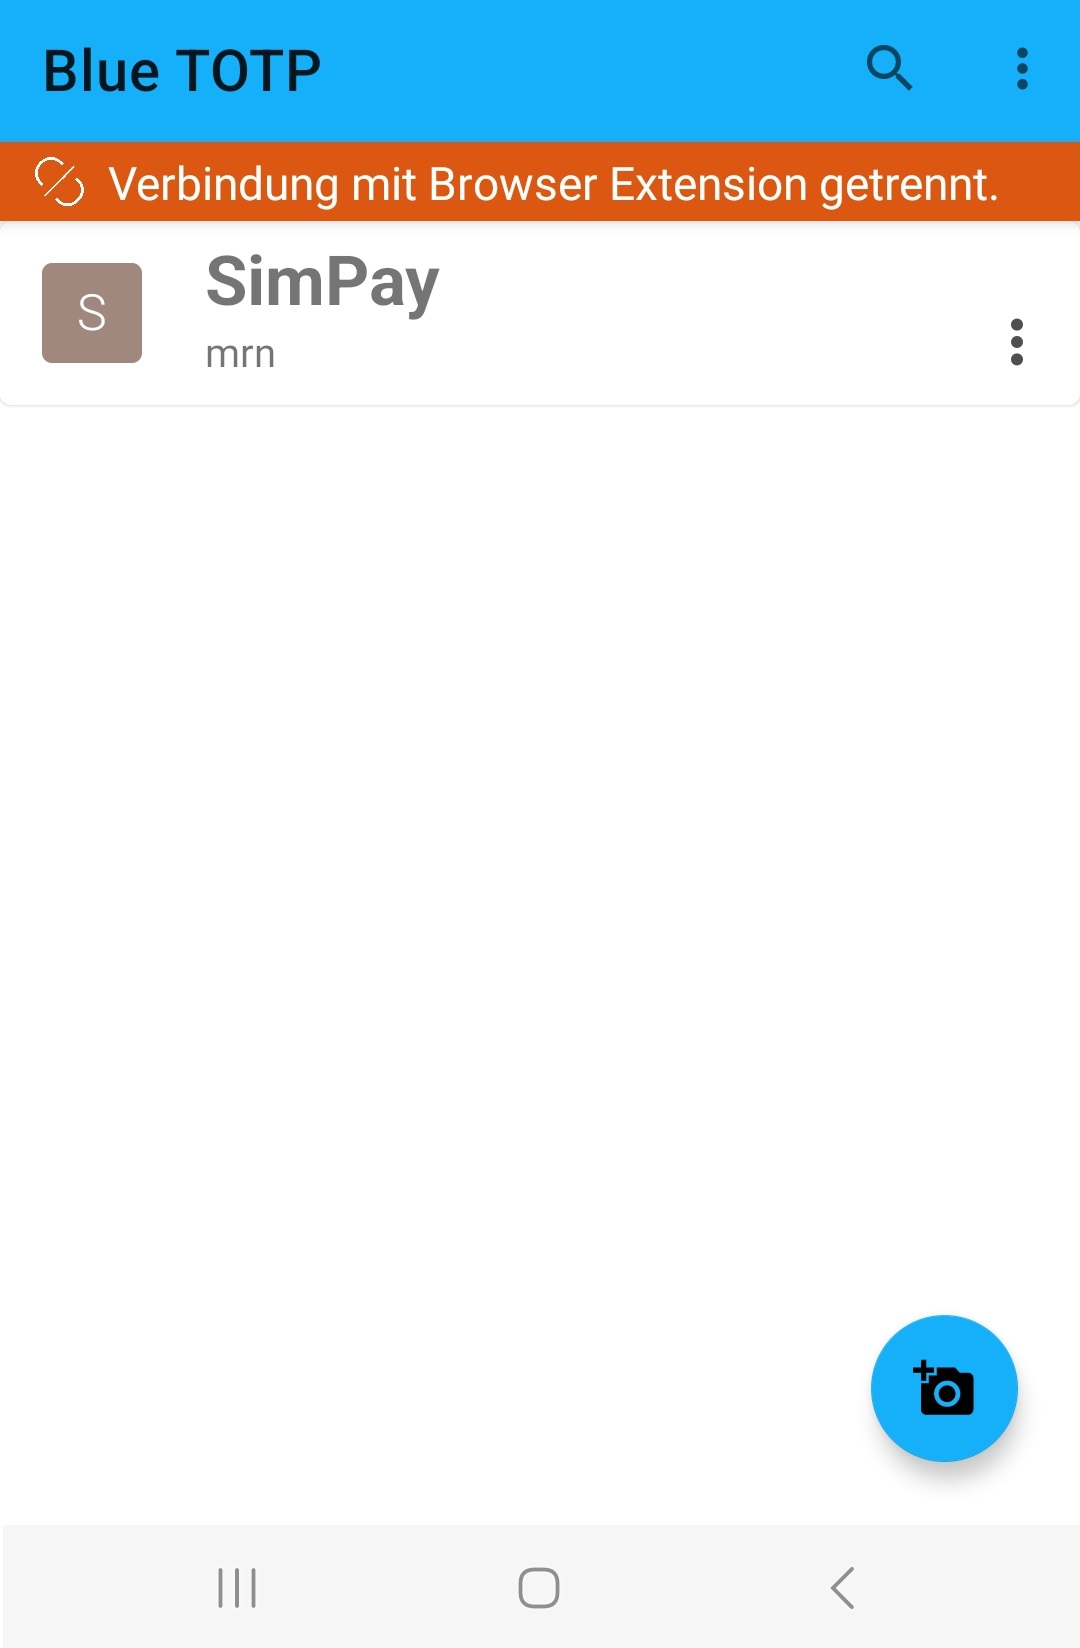
\includegraphics[width=.95\linewidth]{figures/impl/screenshot_app_nicht_verbunden.jpg}
      \caption{Main (nicht verbunden)}
      \label{fig: blue totp app screenshot nicht verbunden}
    \end{subfigure}%
    \begin{subfigure}{.23\textwidth}
      \centering
      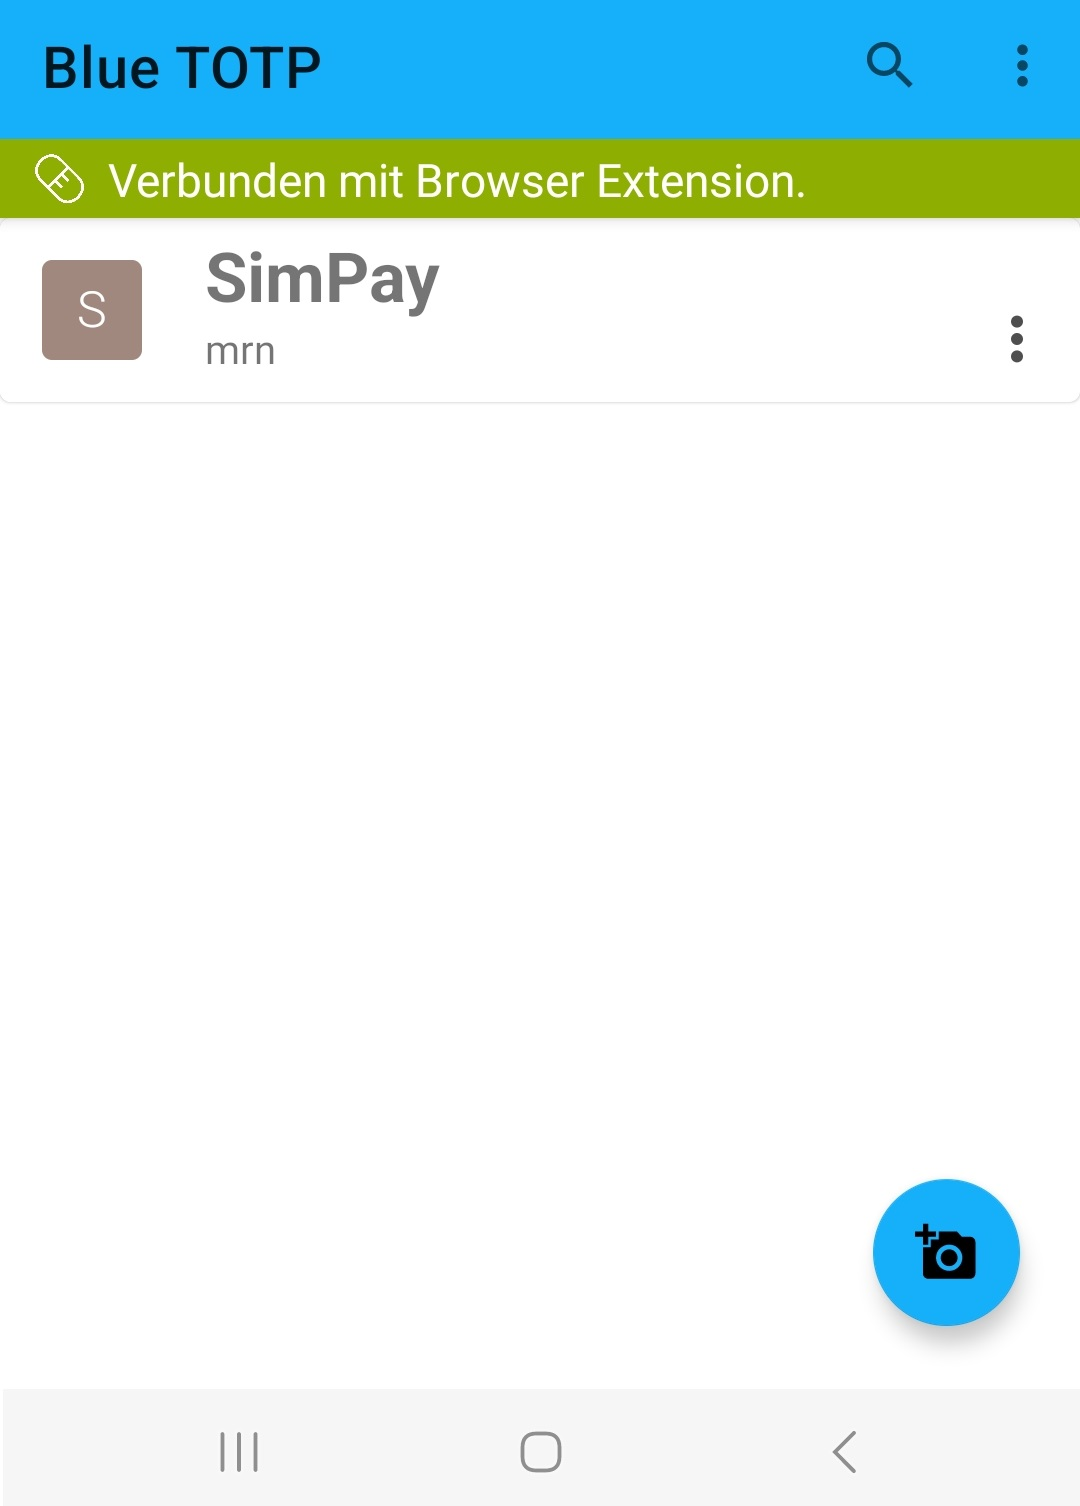
\includegraphics[width=.95\linewidth]{figures/impl/screenshot_app_verbunden.jpg}
      \caption{Main (verbunden)}
      \label{fig: blue totp app screenshot verbunden}
    \end{subfigure}
    \begin{subfigure}{.23\textwidth}
        \centering
        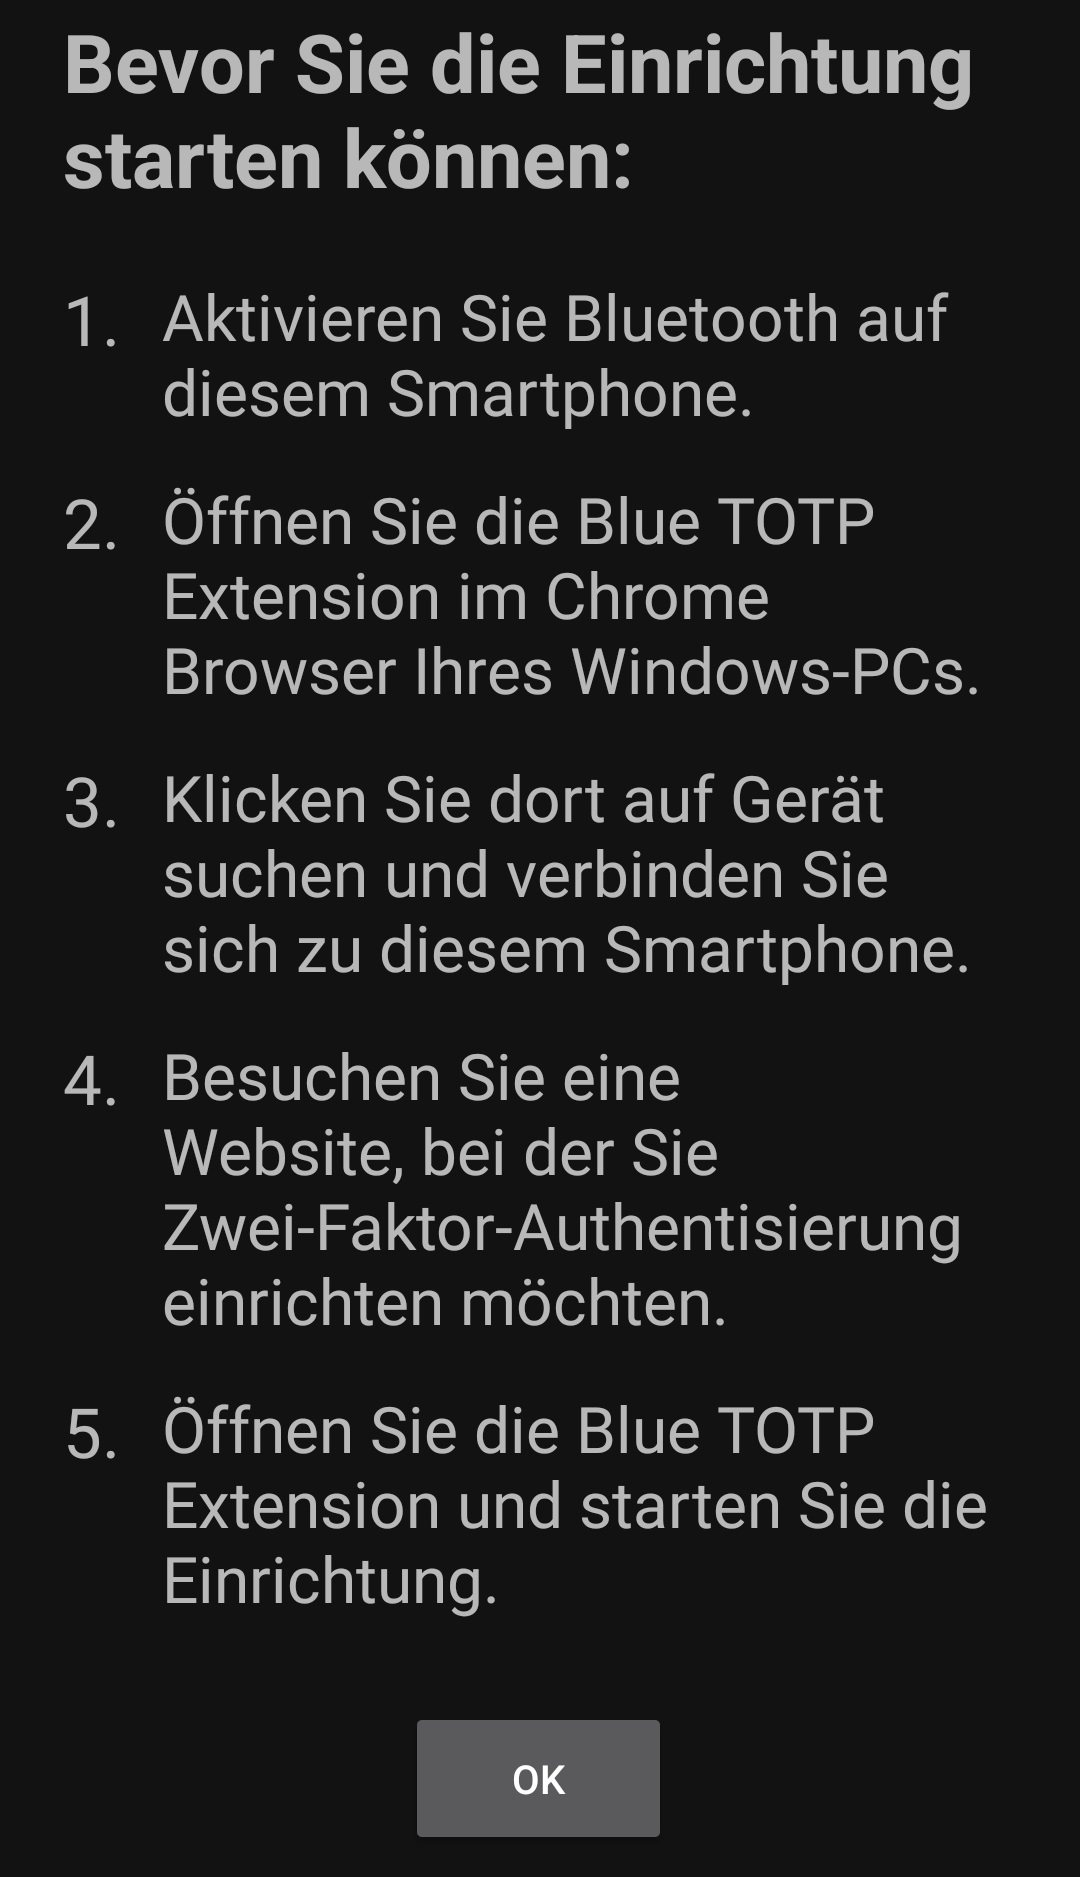
\includegraphics[width=.95\linewidth]{figures/impl/screenshot_app_anleitung.jpg}
        \caption{Anleitung}
        \label{fig: blue totp app screenshot anleitung}
    \end{subfigure}
    \begin{subfigure}{.23\textwidth}
        \centering
        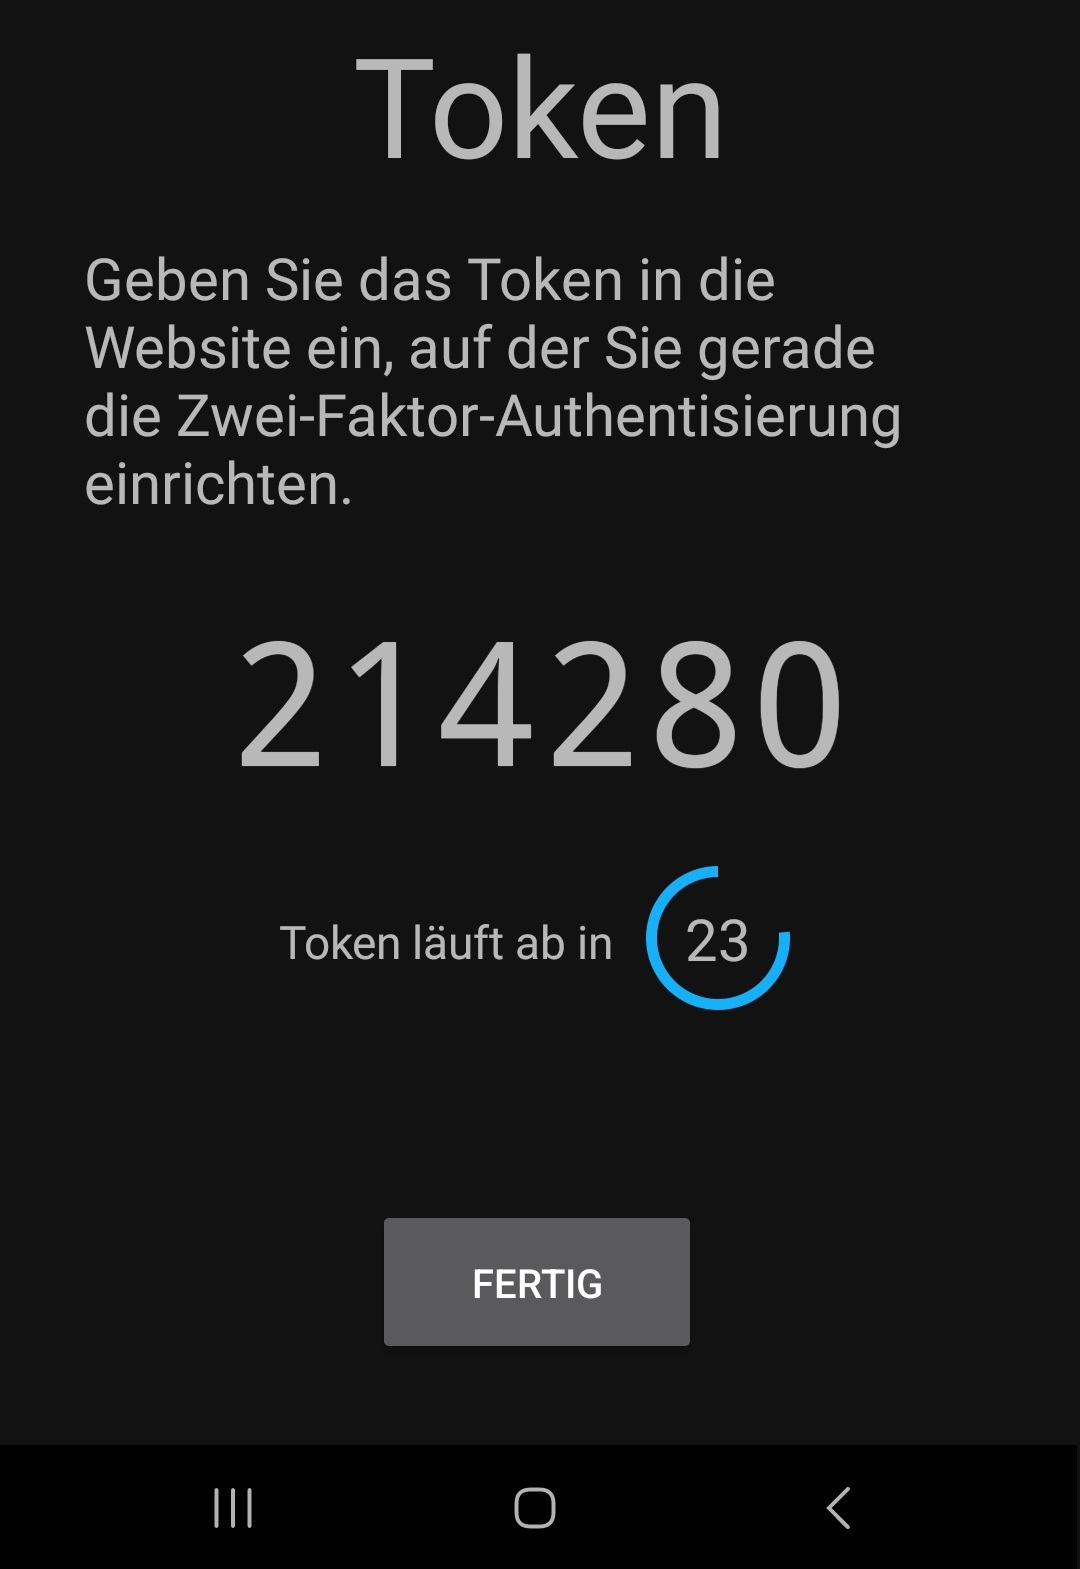
\includegraphics[width=.95\linewidth]{figures/impl/screenshot_app_token.jpg}
        \caption{Token}
        \label{fig: blue totp app screenshot token}
    \end{subfigure}
    \caption[Screens der Blue TOTP App]{Screens/Activities der Blue TOTP App}
    \label{fig: blue totp app screenshots}
\end{figure}

Für den Hintergrundprozess mit der gesamten Bluetooth-Funktionalität wurde ein 
sogenannter Foreground Service gewählt. Auf dem Testgerät konnte dieser tagelang 
laufen und wurde nicht einmal durch Android beendet. Wie bereits erwähnt, variiert 
dieses Verhalten je nach Konfiguration des Android Systems. Leider zeigt diese Art 
von Service permanent eine Notification an, dass die App aktiv ist. Ein passendes 
Beispiel ist ein Music Player. Solange man Musik hört, wird die Notification 
angezeigt und man kann mit dieser sogar interagieren (Musik pausieren, Songs 
überspringen). Für die Blue TOTP App ist der Foreground Service im Nachhinein keine 
gute Wahl. Allerdings ist es nicht leicht (oder nur dem Autor unbekannt), Prozesse 
in Android permanent laufen zu lassen, da es gegen das Prinzip verstößt, 
Arbeitsspeicher, Rechenleistung und Batterie effizient zu verwalten. Der Foreground 
Service schien die einzige plausible Lösung dafür zu sein. Die App wurde 
hauptsächlich mit Android 13 getestet, unterstützt aber auch Android 8.0. 
Allerdings benötigt die Blue TOTP App die Funktion des Bluetooth Low Energy 
Advertisings. Ältere Geräte (auch Geräte mit Android 8.0) verfügen nicht zwingend 
über Bluetooth-Hardware, die diese Funktion unterstützt.